%!TEX TS-program = xelatex
%!TEX encoding = UTF-8 Unicode

\documentclass[a4paper,11pt]{article}


\usepackage{fontspec}

\setmainfont{Linux Libertine}
% \setmainfont{Arial}
% \setmainfont{DejaVu Sans}
% \setmainfont{Georgia}
% \setmainfont{Times New Roman}

\setmonofont{Consolas}[Scale=MatchLowercase]
% \setmonofont{Droid Sans Mono}[Scale=MatchLowercase]
% \setmonofont{Courier New}[Scale=MatchLowercase]

 
\usepackage{listings}
\lstset{%
	language=Java,
	basicstyle=\footnotesize\ttfamily,
	frame=single,
	breaklines=true,
	showstringspaces=false
	}


\usepackage{graphicx}
\graphicspath{ {images/} }

\usepackage{hyperref}

\title{Aggregator Manager}
\author{Καμπυλαυκάς Ιωάννης \\ sdi9500781@di.uoa.gr \and Σούλης Αθανάσιος \\ sdi0900155@di.uoa.gr}
\date{28 Δεκεμβρίου 2015}
\renewcommand{\contentsname}{Περιεχόμενα}
\renewcommand{\figurename}{Σχήμα}

\begin{document}

\begin{sloppypar}

\maketitle

\tableofcontents

\newpage


\section{Το σχήμα της βάσης δεδομένων}



\begin{figure}[h]
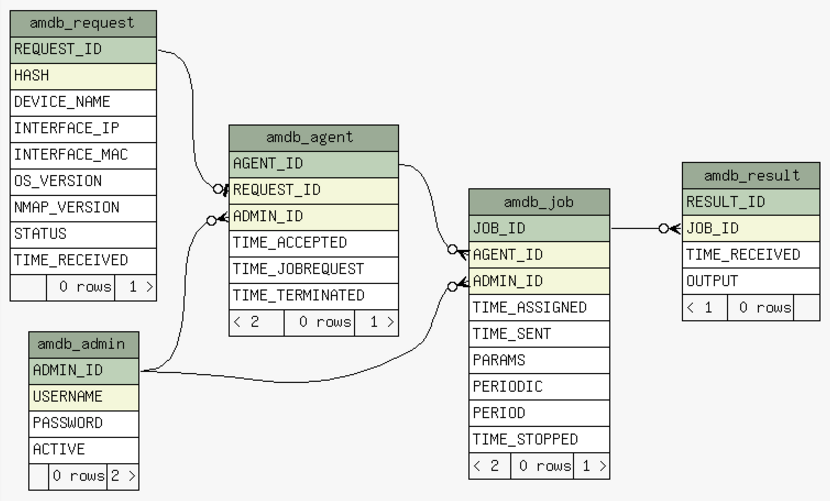
\includegraphics[width=\textwidth]{schema}
\centering
\caption{Το σχήμα της βάσης δεδομένων του Aggregator Manager.}
\end{figure}



\begin{enumerate}


\item amdb\_request

Στον πίνακα αυτό καταγράφονται τα αιτήματα εγγραφής που καταφθάνουν μέσω της σχετικής REST υπηρεσίας.
\begin{itemize}

\item REQUEST\_ID: πρωτεύον κλειδί του πίνακα, δημιουργείται αυτόματα.

\item HASH: το hash των στοιχείων του agent. Για δυο διαφορετικές εγγραφές του πίνακα, οι τιμές του πεδίου αυτού είναι διαφορετικές.

\item DEVICE\_NAME, INTERFACE\_IP, INTERFACE\_MAC, OS\_VERSION, NMAP\_VERSION: τα επιμέρους στοιχεία του agent.

\item STATUS: η κατάσταση του αιτήματος. Μπορεί να έχει μία από τις τιμές: Pending, Accepted, Rejected. 

\item TIME\_RECEIVED: είναι η χρονική στιγμή άφιξης του τελευταίου αιτήματος από κάποιον agent. Αν κάποιος agent στείλει αίτημα με το ίδιο hash δεν δημιουργείται καινούρια εγγραφή αλλά ενημερώνεται το πεδίο αυτό στην ήδη υπάρχουσα εγγραφή.

\end{itemize}

Το πεδίο STATUS είναι πολύ σημαντικό στο σχήμα γιατί βάσει αυτού λαμβάνονται οι περισσότερες αποφάσεις για το πως θα συμπεριφερθεί το σύστημα σε διάφορες καταστάσεις. Την τιμή του πεδίου μπορεί να αλλάξει μόνο κάποιος από τους διαχειριστές, μέσω της γραφικής διεπαφής. Δεν μπορεί να αλλαχτεί από κάποιο εξωτερικό γεγονός, για παράδειγμα λήψη κάποιου αιτήματος μέσω των REST υπηρεσιών. 


\item amdb\_admin

Είναι ο πίνακας των διαχειριστών του συστήματος.
\begin{itemize}

\item ADMIN\_ID: πρωτεύον κλειδί του πίνακα, δημιουργείται αυτόματα από τη βάση δεδομένων.

\item USERNAME: το όνομα χρήστη του διαχειριστή. Υπάρχει περιορισμός μοναδικότητας της τιμής του πεδίου αυτού για τον πίνακα, όπως και στο πεδίο HASH του πίνακα των αιτημάτων.

\item PASSWORD: το συνθηματικό του διαχειριστή. Δεν αποθηκεύεται αυτούσιο το συνθηματικό αλλά η έξοδος του αλγορίθμου SHA256 με είσοδο το συνθηματικό.

\item ACTIVE: το πεδίο αυτό είναι τύπου bit, και ενημερώνεται ανάλογα όταν ο διαχειριστής πραγματοποιήσει είσοδο ή έξοδο από το σύστημα.

\end{itemize}


\item amdb\_agent

Στον πίνακα αυτό καταγράφονται οι agents των οποίων τα αιτήματα για εγγραφή έχουν γίνει αποδεκτά.
\begin{itemize}

\item AGENT\_ID: πρωτεύον κλειδί του πίνακα, δημιουργείται αυτόματα από τη βάση δεδομένων.

\item REQUEST\_ID: ξένο κλειδί στον πίνακα με τα αιτήματα. Επίσης έχει περιορισμό μοναδικής τιμής και σε αυτόν τον πίνακα, που σημαίνει ότι μπορεί να υπάρχει το πολύ ένας agent για κάποιο αίτημα.

\item ADMIN\_ID: ξένο κλειδί στον πίνακα των διαχειριστών. Προσδιορίζει το ποιος διαχειριστής έκανε την έγκριση του αιτήματος.

\item TIME\_ACCEPTED: αντιστοιχεί στη χρονική στιγμή κατά την οποία έγινε δεκτό το αίτημα για εγγραφή.

\item TIME\_JOBREQUEST: αντιστοιχεί στην τελευταία χρονική στιγμή κατά την οποία ο agent έκανε αίτημα για nmap jobs μέσω της σχετικής REST υπηρεσίας, αν το γεγονός αυτό έχει συμβεί.

\item TIME\_TERMINATED: αντιστοιχεί στην χρονική στιγμή κατά την οποία δημιουργήθηκε job τερματισμού για τον agent, αν το γεγονός αυτό έχει συμβεί.

\end{itemize}

Στην περίπτωση που γίνει έγκριση κάποιου αιτήματος για το οποίο ήδη υπάρχει εγγραφή στον πίνακα των agents, τότε δεν δημιουργείται νέα εγγραφή (σύμφωνα και με τον περιορισμό μοναδικότητας του πεδίου REQUEST\_ID) αλλά ενημερώνονται τα πεδία ADMIN\_ID και TIME\_ACCEPTED της υπάρχουσας εγγραφής.


\item amdb\_job

Στον πίνακα αυτό αποθηκεύονται τα nmap jobs που ανατίθενται στους εγκεκριμένους agents.
\begin{itemize}

\item JOB\_ID: πρωτεύον κλειδί του πίνακα, δημιουργείται αυτόματα από τη βάση δεδομένων.

\item AGENT\_ID: ξένο κλειδί στον πίνακα των εγκεκριμένων agents.

\item ADMIN\_ID: ξένο κλειδί στον πίνακα των διαχειριστών. Αντιστοιχεί στον διαχειριστή που έκανε την ανάθεση της εργασίας.

\item TIME\_ASSIGNED: αντιστοιχεί στη χρονική στιγμή της ανάθεσης της εργασίας.

\item TIME\_SENT: είναι η χρονική στιγμή κατά την οποία ο agent έλαβε την εργασία μέσω της σχετικής REST υπηρεσίας, αν το γεγονός αυτό έχει συμβεί.

\item PARAMS: οι παράμετροι του nmap job.

\item PERIODIC: καταγράφει το αν το nmap job είναι περιοδικό η όχι.

\item PERIOD: στην περίπτωση των περιοδικών jobs, καταγράφει το χρονικό διάστημα μεταξύ δυο επαναλήψεων της εργασίας.

\item TIME\_STOPPED: αντιστοιχεί στην πιο πρόσφτατη χρονική στιγμή κατά την οποία δημιουργήθηκε ειδικό job τερματισμού για το συγκεκριμένο nmap job, αν το γεγονός αυτό έχει συμβεί.

\end{itemize}


\item amdb\_result

Στον πίνακα αυτό αποθηκεύονται τα αποτελέσματα των nmap jobs τα οποία καταφθάνουν από τους agents μέσω της σχετικής REST υπηρεσίας.
\begin{itemize}

\item RESULT\_ID: πρωτεύον κλειδί του πίνακα, δημιουργείται αυτόματα από τη βάση δεδομένων.

\item JOB\_ID: ξένο κλειδί στον πίνακα των nmap jobs

\item TIME\_RECEIVED: αντιστοιχεί στη χρονική στιγμή δημιουργίας της εγγραφής του αποτελέσματος (timestamp).

\item OUTPUT: το αποτέλεσμα, δηλαδή η έξοδος του σχετικού nmap job για μια συγκεκριμένη εκτέλεση του.

\end{itemize}

\end{enumerate}


\newpage


\section{Η διαστρωμάτωση του AM}

Η υλοποίηση του Aggregator Manager έχει γίνει χωρίζοντας τον σε επίπεδα, το καθένα με συγκεκριμένες αρμοδιότητες: Data Access Objects (απόκρυψη των λεπτομερειών αποθήκευσης δεδομένων), Caching Control (τοπική αποθήκευση δεδομένων), Service Layer (συνέπεια δεδομένων, business rules του προβλήματος), Model (κλάσεις προς εμφάνιση στη γραφική διεπαφή), Controllers (έλεγχος της διεπαφής και των εμφανιζόμενων δεδομένων), Views (υλοποίηση όψεων διεπαφής) και τέλος REST (υπηρεσίες επικοινωνίας με τους Software Agents). Η διαστρωμάτωση παρουσιάζεται παρακάτω:
\\

\begin{figure}[h]
% 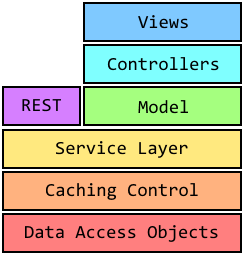
\includegraphics[width=\textwidth]{layers}
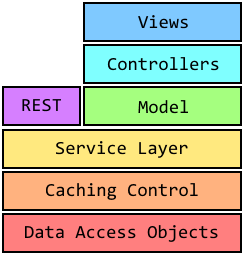
\includegraphics[width=9cm]{layers}
\centering
\end{figure}

\newpage


\subsection{Data Access Layer (Dao)}

Αποτελείται από τις κλάσεις RequestDao, AdminDao, AgentDao, JobDao, ResultDao οι οποίες αντιστοιχούν στις οντότητες του προβλήματος. Ευθύνη του επιπέδου αυτού είναι να κρύψει τις λεπτομέρειες της αποθήκευσης στην υποκείμενη αποθήκη δεδομένων, που στην περίπτωση μας είναι μια σχεσιακή βάση δεδομένων. Κάθε κλάση του επιπέδου αυτού αποτελείται από στατικές μεθόδους οι οποίες υλοποιούν την πρόσβαση στην αποθήκη δεδομένων. Οι μέθοδοι αυτές δεν κάνουν κάποιο έλεγχο ορθότητας των παραμέτρων τους ή συνέπειας των δεδομένων, αφού η αρμοδιότητα αυτή ανήκει σε ανώτερο επίπεδο. Υποθέτωντας ότι η χρήση της είναι σωστή, κάθε μέθοδος ουσιαστικά εκτελεί ένα απλό ερώτημα SQL στην υποκείμενη βάση δεδομένων και επιστρέφει τα αποτελέσματα στο αμέσως ανώτερο επίπεδο. Για την επιστροφή των αποτελεσμάτων χρησιμοποιούνται instances της κάθε κλάσης. Τα μη στατικά μέλη της κάθε κλάσης είναι τα πεδία που αντιστοιχούν στις στήλες του κάθε πίνακα της βάσης δεδομένων καθώς και οι getters/setters για αυτά.

\subsection{Caching Control Layer (CC)}

Αποτελείται από τις κλάσεις RequestCC, AdminCC, AgentCC, JobCC, ResultCC. Κάθε κλάση προσφέρει μεθόδους πρόσβασης οι οποίες διατηρούν όμοια τη διεπαφή του Dao επιπέδου. Η πρόσθετη λειτουργία που εισάγει το επίπεδο αυτό είναι η τοπική αποθήκευση (caching) των αποτελεσμάτων που έρχονται από το Dao επίπεδο. Η τοπική αποθήκευση γίνεται με τη βοήθεια των κλάσεων RequestCache, AdminCache, AgentCache, JobCache, ResultCache. Ένα στιγμιότυπο της κάθε μιας από αυτές έχει την ευθύνη να αποθηκεύει τοπικά τις αναφορές που επιστρέφονται από το αντίστοιχο Dao επίπεδο. Για την υλοποίηση των cache κλάσεων χρησιμοποιήθηκε μια τροποποιημένη δομή κατακερματισμού με συνδεδεμένη λίστα (LRUHashMap) η οποία προσφέρει, πέρα από τη δυνατότητα ανάκτησης αναφορών σε σταθερό χρόνο, και τη διατήρησή των αναφορών σε σειρά ανάλογα με το πότε έγινε τελευταία φορά χρήση τους (τοποθέτηση ή ανάκτηση). Το επίπεδο τοπικής αποθήκευσης προσφέρει τη δυνατότητα απενεργοποίησης του. Στην περίπτωση αυτή, οι μέθοδοι του επιπέδου απλά προωθούν τις κλήσεις στο Dao επίπεδο και επιστρέφουν τα αποτελέσματά από αυτό χωρίς να προβούν σε κάποια άλλη ενέργεια.

\subsection{Service Layer (Srv)}

Αποτελείται από τις κλάσεις RequestSrv, AdminSrv, AgentSrv, JobSrv, ResultSrv. Κύρια ευθύνη του επιπέδου είναι η διασφάλιση της συνέπειας των δεδομένων και η σωστή χρήση των CC/Dao επιπέδων σύμφωνα με τη λογική του προβλήματος έτσι ώστε να αποφεύγονται εντελώς τα σφάλματα σε αυτά τα δυο επίπεδα. Μέσω του Srv επιπέδου, τα μόνα σφάλματα που μπορεί να συμβούν στα δύο κατώτερα επίπεδα είναι απρόσμενα σφάλματα (π.χ. μια αποσύνδεση από τη βάση δεδομένων) και όχι λογικά σφάλματα η σφάλματα σε ερωτήματα. Μια κλάση του Srv επιπέδου μπορεί να χρησιμοποιεί περισσότερες από μια κλάσεις των υποκείμενων επιπέδων για να παρέχει τις υπηρεσίες της. Το Srv επίπεδο χρησιμοποιεί exceptions (τύπου SrvException) για να ειδοποιήσει τα ανώτερα επίπεδα για λογικά σφάλματα ή σφάλματα πρόσβασης δεδομένων από τα κατώτερα επίπεδα. Πέρα από τον έλεγχο της ορθότητας των παραμέτρων και της ευθυγράμμισης με τη λογική του προβλήματος, το επίπεδο υλοποιεί συγχρονισμό στην πρόσβαση των επιμέρους αποθηκών δεδομένων των κατωτέρων επιπέδων. Η λογική αυτή είναι απαραίτητη για να δημιουργηθούν σωστά πιο σύνθετες ενέργειες από τις απλές ενέργειες πρόσβασης δεδομένων του Dao επιπέδου.

\subsection{Controllers-Model}
Χρήση των υπηρεσιών του Srv επιπέδου κάνουν δύο επίπεδα: Το επίπεδο των REST υπηρεσιών και το επίπεδο των Controllers που αντιστοιχούν στις διάφορες όψεις της γραφικής διεπαφής. Το επίπεδο Srv είναι το τελευταίο επίπεδο στο οποίο επιστρέφονται Dao αντικείμενα ως αποτελέσματα. Κάθε Controller χρησιμοποιώντας Dao αντικείμενα από το Srv επίπεδο, δημιουργεί αντικείμενα του Model επιπέδου τα οποία εμφανίζει στην αντίστοιχη όψη. Το Model επίπεδο περιέχει κλάσεις που αντιστοιχούν και αυτές στις οντότητες του προβλήματος, έχουν όμως κύριο σκοπό το να εξυπηρετήσουν την εμφάνιση των δεδομένων στις διάφορες όψεις. Για το λόγο αυτό, τα διάφορα πεδία τους υλοποιούνται από JavaFX properties και οι συλλογές τέτοιων αντικειμένων μέσα στους Controllers είναι observable JavaFX συλλογές έτσι ώστε αλλαγές στα πεδία των αντικειμένων ή στις συλλογές να αντικατοπτρίζονται στην εκάστοτε όψη της διεπαφής. Οι κλάσεις του Model επιπέδου μπορεί να ενσωματώνουν και πρόσθετα στοιχεία πέρα από αυτά των οντοτήτων στις οποίες αντιστοιχούν. Για παράδειγμα η κλάση Agent περιέχει πεδίο requestHashProperty, πληροφορία που βρίσκεται στο RequestDao και όχι στο AgentDao αντικείμενο που επιστρέφεται από το Srv επίπεδο. Η πληροφορία αυτή περνιέται στον constructor του Agent κατά τη δημιουργία του, συνδυάζοντας πληροφορίες από δύο σχετικά Dao αντικείμενα και επιτρέποντας την εύκολη απεικόνιση της επιθυμητής πληροφορίας.

\subsection{Views}
Είναι το επίπεδο των όψεων της γραφικής διεπαφής. Η περιγραφή των όψεων έχει γίνει με FXML, και υπάρχει αντιστοίχιση της κάθε όψης με έναν Controller που αναλαμβάνει τον έλεγχο των δεδομένων που θα εμφανιστούν στη διεπαφή ή θα δημιουργηθούν από αυτή.

\newpage


\section{Μια πιο κοντινή ματιά στα κατώτερα επίπεδα του AM}

\subsection{Data Access Objects}

Ακολουθούν οι κύριες, στατικές μέθοδοι του επιπέδου για τα αντικείμενα Agent:

\begin{lstlisting}
public class AgentDao {

    public static long create(long requestId, long adminId, Date timeAccepted) throws DaoException;

    public static AgentDao findById(long agentId) throws DaoException;
    public static AgentDao findByRequestId(long requestId) throws DaoException;

    public static Set<AgentDao> findAllWithAdminId(long adminId) throws DaoException;
    public static Set<AgentDao> findAll() throws DaoException;
    public static Set<AgentDao> findAllWithRequestStatus(RequestStatus requestStatus) throws DaoException;

    public static void update(long agentId, long adminId, Date timeAccepted)throws DaoException;
    public static void setTimeJobRequest(long agentId, Date timeJobRequest) throws DaoException;
    public static void setTimeTerminated(long agentId, Date timeTerminated) throws DaoException;
}

\end{lstlisting}

Η μέθοδος create() δημιουργεί ένα καινούριο Agent με τις παρεχόμενες πληροφορίες. Πέρα από τις πληροφορίες του ίδιου του Agent, πρέπει να της περαστούν ως παράμετροι οι αριθμοί ταυτότητας ενός Request (για το οποίο δημιουργείται ο Agent) και ενός Admin (ο οποίος δημιουργεί τον Agent). Η μέθοδος δεν κάνει έλεγχο εγκυρότητας των παραπάνω πληροφοριών, όπως αναφέρθηκε νωρίτερα. Υποθέτει ότι το Request και ο Admin υπάρχουν στην αποθήκη δεδομένων και ότι βρίσκονται σε έγκυρη κατάσταση για τη δημιουργία ενός Agent. Η μέθοδος επιστρέφει τον αριθμό ταυτότητας του Agent που δημιουργήθηκε. Οι μέθοδοι findById() και findByRequestId() αναζητούν την αποθήκη των Agents βάσει του αριθμού ταυτότητας που παρέχεται και επιστρέφουν ένα αντικείμενο AgentDao ή null στην περίπτωση που δε βρεθεί ο Agent. Οι μέθοδοι findAllWithAdminId(), findAll(), findAllWithRequestStatus() επιστρέφουν σύνολα από Agents που πληρούν τις προδιαγραφές των μεθόδων. Οι μεθοδοι update(), setTimeJobRequest(), setTimeTerminated() μεταβάλλουν υπάρχοντες Agents. Και πάλι, υποθέτουν ότι οι αριθμοί ταυτότητας των Agents είναι σωστοί, αντιστοιχούν δηλαδή σε υπάρχοντα Agent και κάνουν την αλλαγή σε αυτόν. Δεν επιστρέφουν κάποια boolean τιμή αφού η αλλαγή υποτίθεται οτι είναι πάντα επιτυχής δεδομένου ότι έχουμε έγκυρους αριθμούς ταυτότητας. Στην περίπτωση οποιουδήποτε σφάλματος πρόσβασης δεδομένων, αυτές οι μέθοδοι αποτυγχάνουν με DaoException, όπως και όλες οι προηγούμενες.

\newpage

Παρακάτω παρουσιάζεται ως παράδειγμα ο κώδικας της μεθόδου create() για τους Agents:
\begin{lstlisting}
public static long create(long requestId, long adminId, Date timeAccepted) throws DaoException {

    String sql = new StringBuilder()
            .append("insert into amdb_agent ")
            .append("(REQUEST_ID, ADMIN_ID, TIME_ACCEPTED) ")
            .append("values ")
            .append("(?, ?, ?)")
            .toString();

    try (SynchronizedStatement ss = ConnectionSingleton.getInstance().getStatement(sql)) {

        log.debug("");
        log.debug("Executing query: " + sql);

        log.debug("Setting parameter 1 to: " + requestId);
        ss.setLong(1, requestId);

        log.debug("Setting parameter 2 to: " + adminId);
        ss.setLong(2, adminId);

        log.debug("Setting parameter 3 to: " + timeAccepted);
        ss.setTimestamp(3, new Timestamp(timeAccepted.getTime()));

        int rows = ss.executeUpdate();
        log.debug(rows + (rows == 1 ? " row " : " rows ") + "inserted.");

        ResultSet rs = ss.getGeneratedKeys();

        if (!rs.next())
            throw new DaoException("Could not retrieve id for created agent.");

        long id = rs.getLong(1);
        log.debug("Id returned: " + id);

        return id;

    } catch (SQLException e) {
        // e.printStackTrace();
        log.error(e.getMessage());

        throw new DaoException("Error while creating agent with requestId: " + requestId);
    }
}
\end{lstlisting}

Ο κύκλος ζωής μιας μεθόδου του επιπέδου Dao είναι πολύ απλός. Ουσιαστικά πρόκειται για τη δημιουργία ενός SynchronizedStatement, των προσδιορισμό των παραμέτρων του, την εκτέλεση του statement και τη λήψη των αποτελεσμάτων. Στο τέλος της μεθόδου το statement κλείνει (υλοποιεί το interface AutoCloseable) και μπορεί να γίνει κλήση μιας οποιαδήποτε άλλης μεθόδου του Dao επιπέδου.

Η κλάση SynchronizedStatement δεν είναι παρά ένας wrapper για την κλάση PreparedStatement του JDBC και οι μέθοδοι που εκτελούνται πάνω στην SynchronizedStatement προωθούνται στο περιεχόμενο PreparedStatement αντικείμενο. Η κλάση SynchronizedStatement όμως έχει ένα πρόσθετο χαρακτηριστικό. Μέσω ενός στατικού σημαφόρου με αρχική τιμή 1, μόνο ένα SynchronizedStatement μπορεί να είναι ενεργό κάθε φορά. Η διάρκεια ζωής ενός SynchronizedStatement είναι από τη στιγμή της κατασκευής του (constructor, Semaphore.acquire()) έως τη στιγμή που κλείνει (close(), Semaphore.release()). Με αυτό το μηχανισμό, πολλά νήματα μπορούν να καλούν ταυτόχρονα μεθόδους του Dao επιπέδου, με την εγγύηση ότι μόνο ένα Statement θα χρησιμοποιείται κάθε φορά και μόνο όταν αυτό κλείσει να μπορέσει να χρησιμοποιηθεί το επόμενο, ακριβώς σαν να είχαμε μόνο ένα νήμα με πρόσβαση στο Dao επίπεδο.

Ακολουθεί ένα μέρος της κλάσης SynchronizedStatement:

\begin{lstlisting}
public class SynchronizedStatement implements AutoCloseable {

    private PreparedStatement ps;

    private static Semaphore sem = new Semaphore(1);

    public SynchronizedStatement(Connection connection, String sql) throws InterruptedException {

        sem.acquire();

        try {
            ps = connection.prepareStatement(sql, Statement.RETURN_GENERATED_KEYS);
        } catch (SQLException e) {
            ps = null;
        }
    }

    public void setString(int parameterIndex, String x) throws SQLException
    {
        ps.setString(parameterIndex, x);
    }

    public void setInt(int parameterIndex, int x) throws SQLException {
        ps.setInt(parameterIndex, x);
    }

    public void setLong(int parameterIndex, long x) throws SQLException {
        ps.setLong(parameterIndex, x);
    }



    public void setBoolean(int parameterIndex, boolean x) throws SQLException {
        ps.setBoolean(parameterIndex, x);
    }

    public void setDate(int parameterIndex, Date x) throws SQLException {
        ps.setDate(parameterIndex, x);
    }

    public void setTimestamp(int parameterIndex, Timestamp x) throws SQLException {
        ps.setTimestamp(parameterIndex, x);
    }

    public ResultSet executeQuery() throws SQLException {
        return ps.executeQuery();
    }

    public int executeUpdate() throws SQLException {
        return ps.executeUpdate();
    }

    ResultSet getResultSet() throws SQLException {
        return ps.getResultSet();
    }

    ResultSet getGeneratedKeys() throws SQLException {
        return ps.getGeneratedKeys();
    }

    @Override
    public void close() throws SQLException {

        ps.close();

        sem.release();
    }
}

\end{lstlisting}

Η σύνδεση που χρησιμοποιείται στον constructor του PreparedStatement είναι ένα Singleton τύπου java.sql.Connection που βρίσκεται στο Dao επίπεδο. Η χρήση του SynchronizedStatement κρίθηκε απαραίτητη λόγω του ότι εξασφαλίζει απόλυτα πως δυο νήματα θα εκτελέσουν διαδοχικά και εξ' ολοκλήρου μεθόδους πάνω σε δυο ξεχωριστά PreparedStatement αντικείμενα που προέρχονται από την ίδια σύνδεση. Χωρίς το SynchronizedStatement, και επειδή ο JDBC driver ενδέχεται να αποθηκεύει εσωτερικά PreparedStatement αντικείμενα, μπορεί να επιστρέψει το ίδιο αντικείμενο (για το ίδιο SQL ερώτημα) σε δυο διαφορετικά νήματα, τα οποία θα εκτελούν ταυτόχρονα μεθόδους στο ίδιο PreparedStatemenτ με απρόβλεπτα αποτελέσματα. \url{https://docs.oracle.com/cd/B10501_01/java.920/a96654/stmtcach.htm#1069943}


\newpage

\subsection{Caching Control Layer}

Το επίπεδο ελέγχου τοπικής αποθήκευσης λειτουργεί με μια απλή λογική. Κάθε οντότητα που αποθηκεύεται στην υποκείμενη αποθήκη δεδομένων ταυτοποιείται από έναν αριθμό. Επίσης βάσει των κανόνων του προβλήματος, ενδέχεται μια τιμή ενός πεδίου της οντότητας να είναι μοναδική, για παράδειγμα το username ενός Admin. Το επίπεδο τοπικής αποθήκευσης εκθέτει χωρίς αλλαγές το interface του αντίστοιχου Dao επιπέδου, και καθώς πληροφορίες έρχονται από το Dao επίπεδο, αποθηκεύονται τοπικά για άμεση πρόσβαση αργότερα από το ανώτερο επίπεδο. Οι μέθοδοι του επιπέδου χωρίζονται κι εδώ σε μεθόδους δημιουργίας οντότητας, αναζήτησης οντότητας, αναζήτησης συνόλου οντοτήτων και ενημέρωσης οντότητας. Παρουσιάζεται ως παράδειγμα η υλοποίηση του επιπέδου για τους Agents, η υλοποίηση είναι ανάλογη και για τις υπόλοιπες οντότητες.

\subsubsection{Δημιουργία}

\begin{lstlisting}
public static long create(long requestId, long adminId, Date timeAccepted) throws DaoException {

    if (cacheDisabled())
        return AgentDao.create(requestId, adminId, timeAccepted);
        
    long agentId = AgentDao.create(requestId, adminId, timeAccepted);

    AgentDao ad = AgentDao.findById(agentId);

    if (ad == null)
        return 0;

    cache.put(ad);

    return ad.getAgentId();
}
\end{lstlisting}

Αρχικά γίνεται έλεγχος για το αν το επίπεδο τοπικής αποθήκευσης είναι ενεργό. Αν αυτό δε συμβαίνει, η κλήση απλά προωθείται στο κατώτερο Dao επίπεδο. Αν η τοπική αποθήκευση είναι ενεργή, τότε μετά τη δημιουργία της νέας οντότητας, αυτή αποθηκεύεται στην cache για γρήγορη ανάκτηση πριν επιστραφεί ο αριθμός ταυτότητας.

\newpage


\subsubsection{Αναζήτηση οντότητας}

\begin{lstlisting}
public static AgentDao findById(long agentId) throws DaoException {

    if (cacheDisabled())
        return AgentDao.findById(agentId);

    AgentDao ad = cache.getById(agentId);

    if (ad != null)
        return ad;

    ad = AgentDao.findById(agentId);

    if (ad != null)
        cache.put(ad);
        
    return ad;
}
\end{lstlisting}

Μετά τον έλεγχο για το αν το επίπεδο γίνεται ενεργό, αντί να γίνει πρόσβαση στην υποκείμενη αποθήκη δεδομένων μέσω του Dao επιπέδου, γίνεται προσπάθεια να βρεθεί η ζητούμενη αναφορά στην τοπική αποθήκη. Αν η αναζήτηση είναι επιτυχής τότε η αναφορά επιστρέφεται από την τοπική αποθήκη. Αν όχι, τότε γίνεται αναζήτηση στην υποκείμενη αποθήκη. Και οι δύο ενέργειες πάνω στην τοπική αποθήκη getById() και put() έχουν σαν αποτέλεσμα η αναφορά που ανακτήθηκε ή αποθηκεύτηκε να γίνει η πιο πρόσφατα χρησιμοποιημένη αναφορά της τοπικής αποθήκης δεδομένων. Αυτό είναι αναγκαίο στην περίπτωση που η τοπική αποθήκη έχει μέγιστο μέγεθος, για να επιλέγει την παλαιότερα χρησιμοποιημένη αναφορά για διαγραφή όταν το μέγεθος της αποθήκης φτάσει το μέγιστο και ζητηθεί προσθήκη μιας νέας αναφοράς. Πέρα από τη μέθοδο findById(), στην κλάση AgentCC υπάρχει και η μέθοδος findByRequestId() για αναζήτηση οντότητας Agent με βάση το μοναδικό αριθμό ταυτότητας requestId για κάθε Agent. Η μέθοδος findByRequestId() είναι ακριβώς ανάλογη της findById() με τη μόνη διαφορά ότι σε αυτή γίνονται κλήσεις AgentDao.findByRequestId() και AgentCache.getByRequestId().

\newpage


\subsubsection{Αναζήτηση συνόλου οντοτήτων}

\begin{lstlisting}
public static Set<AgentDao> findAllWithAdminId(long adminId) throws DaoException {

    if (cacheDisabled())
        return AgentDao.findAllWithAdminId(adminId);

    Set<AgentDao> agents = AgentDao.findAllWithAdminId(adminId);

    for (AgentDao ad : agents)
        cache.put(ad);

    return agents;
}
\end{lstlisting}

Η παραπάνω μέθοδος βρίσκει όλους τους Agents που έχουν εγκριθεί από συγκεκριμένο Admin. Γίνεται αναζήτηση της υποκείμενης αποθήκης δεδομένων, και τα αποτελέσματα εισάγονται με τη σειρά στην τοπική αποθήκη δεδομένων για γρήγορη ανάκτηση αργότερα. Μετά την εισαγωγή, το πιο πρόσφατα χρησιμοποιημένο αντικείμενο της τοπικής αποθήκης είναι το τελευταίο αντικείμενο που εισήχθη σε αυτήν. Ο λόγος που έχουμε πάντα πρόσβαση στην υποκείμενη αποθήκη δεδομένων είναι ότι δεν υπάρχει εύκολος τρόπος να γνωρίζουμε ότι η τοπική αποθήκη περιέχει όλα τα αντικείμενα που ικανοποιούν συγκεκριμένα κριτήρια. Μετά την εισαγωγή στην τοπική αποθήκη, το σύνολο των αντικειμένων επιστρέφεται στο ανώτερο επίπεδο. Πέρα από τη μέθοδo findAllWithAdminId() στην κλάση AgentCC υπάρχουν και οι μέθοδοι findAll() και findAllWithRequestStatus() για την αναζήτηση συνόλου Agent οντοτήτων.

\newpage


\subsubsection{Μεταβολή οντότητας}

\begin{lstlisting}
public static void setTimeTerminated(long agentId, Date timeTerminated) throws DaoException {

    if (cacheDisabled()) {
        AgentDao.setTimeTerminated(agentId, timeTerminated);
        return;
    }

    try {

        AgentDao.setTimeTerminated(agentId, timeTerminated);

        AgentDao ad = cache.getById(agentId);

        if (ad == null)
            return;

        ad.setTimeTerminated(timeTerminated);

    } catch (DaoException e) {

        cache.deleteById(agentId);

        throw e;
    }
}
\end{lstlisting}

Η μέθοδος setTimeTerminated) αλλάζει το χρόνο τερματισμού ενός Agent. Στην περίπτωση μεταβολής υπάρχουσας οντότητας, αρχικά καλείται η αντίστοιχη μέθοδος του Dao επιπέδου για να ενημερώσει την αποθηκευμένη στην υποκείμενη αποθήκη οντότητα. Συνεπώς θα μπορούσαμε να πούμε ότι το επίπεδο της τοπικής αποθήκευσης έχει μια write-through λογική όσον αφορά τις μεταβολές οντοτήτων. Ακολούθως, γίνεται έλεγχος για το αν η οντότητα που μεταβλήθη βρίσκεται στην τοπική αποθήκη. Στην περίπτωση που αυτό συμβαίνει, τότε αλλάζει κατάλληλα ο χρόνος τερματισμού και για την τοπικά αποθηκευμένη αναφορά, έτσι ώστε η τοπική αποθήκη να παραμείνει συνεπής με την υποκείμενη αποθήκη. Η κλήση της AgentCache.getById() έχει και πάλι σαν αποτέλεσμα η οντότητα που μεταβλήθηκε να γίνει η πιο πρόσφατα χρησιμοποιημένη της τοπικής αποθήκης. Στην περίπτωση που το Dao επίπεδο αποτύχει με κάποιο DaoException, τυχόν τοπικά αποθηκευμένη αναφορά διαγράφεται από την τοπική αποθήκη αφού δε γνωρίζουμε ποια είναι πλέον η κατάσταση του αντικειμένου στην υποκείμενη αποθήκη.

\newpage


\subsubsection{Η υλοποίηση της τοπικής αποθήκευσης}

\begin{lstlisting}
public class AgentCache {

    private LRUHashMap<Long, AgentDao> cacheAgentId;
    private LRUHashMap<Long, AgentDao> cacheRequestId;

    public AgentCache() {

        cacheAgentId = new LRUHashMap<Long, AgentDao>();
        cacheRequestId = new LRUHashMap<Long, AgentDao>();
    }

    public synchronized void clear() {

        cacheAgentId.clear();
        cacheRequestId.clear();
    }

    public synchronized void put(AgentDao ad) {

        cacheAgentId.put(ad.getAgentId(), ad);
        cacheRequestId.put(ad.getRequestId(), ad);
    }

    public synchronized AgentDao getById(long agentId) {

        return cacheAgentId.get(agentId);
    }

    public synchronized AgentDao getByRequestId(long requestId) {

        return cacheRequestId.get(requestId);
    }

    public synchronized void deleteById(long agentId) {

        AgentDao ad = cacheAgentId.remove(agentId);
        if (ad == null)
            return;

        cacheRequestId.remove(ad.getRequestId());
    }

    public synchronized void deleteByRequestId(long requestId) {

        AgentDao ad = cacheRequestId.remove(requestId);
        if (ad == null)
            return;

        cacheAgentId.remove(ad.getAgentId());
    }
}
\end{lstlisting}

\newpage

Ο παραπάνω κώδικας δείχνει την υλοποίηση της τοπικής αποθήκευσης για την κλάση AgentCC. Για την κλάση AgentCC υπάρχουν δύο τρόποι αναζήτησης αναφορών τύπου AgentDao, με βάση το agent id του στιγμιοτύπου και με βάση το request id του στιγμιοτύπου, αφού αυτά είναι τα πεδία που είναι μοναδικά για κάθε Agent. Για τον λόγο αυτό χρησιμοποιούνται δυο στιγμιότυπα της κλάσης LRUHashMap που παρουσιάζεται αμέσως παρακάτω. Η μέθοδος clear() αδειάζει και τα δύο στιγμιότυπα από όλες τις αποθηκευμένες αναφορές. Η μέθοδος put() τοποθετεί μια αναφορά και στα δύο hash maps, στην πρώτη περίπτωση με κλειδί το agent id και στη δεύτερη με κλειδί το request id. Οι μέθοδοι getById() και getByRequestId() επιστρέφουν αναφορές βάσει του agent id και βάσει του request id αντίστοιχα. Οι μέθοδοι deleteById() και deleteByRequestId() διαγράφουν από το ένα hash map με βάση το κλειδί που περνιέται ως παράμετρος, και φροντίζουν να διαγράψουν και από το άλλο hash map αφού έχουν ανακτήσει το κλειδί για αυτό, κρατώντας έτσι τα δύο hash maps πάντα συγχρονισμένα όσον αφορά το ποιές αναφορές περιέχουν. Όλες οι μέθοδοι είναι synchronized αφού η δομή LRUHashMap δεν είναι ασφαλής στη χρήση από πολλά νήματα. Η υλοποίησή της βασίζεται στη γενικευμένη δομή LinkedHashMap<K,V> του java.util package.

Οι αλλαγές που έχουν γίνει σε αυτή φαίνονται παρακάτω:

\begin{lstlisting}
public class LRUHashMap<K, V> extends LinkedHashMap<K, V> {

    private long maxSize;

    public LRUHashMap() {
        super();
        this.maxSize = 0;
    }

    public LRUHashMap(long maxSize) {
        super();
        this.maxSize = maxSize;
    }

    @Override
    public V put(K key, V value) {
        if (maxSize > 0)
            remove(key);

        return super.put(key, value);
    };

    @Override
    public V get(Object key) {
        V value = super.get(key);

        if (value != null)
            put((K) key, value);

        return value;
    };
    @Override
    protected boolean removeEldestEntry(Entry<K, V> eldest) {
        if (maxSize == 0)
            return false;

        return this.size() > maxSize;
    }
}
\end{lstlisting}

Ο πρώτος constructor δημιουργεί ένα LRUHashMap χωρίς περιορισμό στο μέγεθος κάνοντας αδιάφορη την LRU λογική. Ο δεύτερος περιορίζει το μέγεθος του map σε συγκεκριμένο μέγιστο. Η μέθοδος removeEldestEntry() εκτελείται κάθε φορά που εισάγεται μια καινούρια αντιστοίχιση κλειδιού-τιμής στο hash map. Επιστρέφει true αν το μέγεθος του hash map έχει ξεπεράσει το μέγιστο, έτσι ώστε να γίνει διαγραφή του λιγότερο πρόσφατα χρησιμοποιημένου κλειδιού. Η μέθοδος put() έχει αλλαχτεί έτσι ώστε στην περίπτωση που ένα κλειδί υπάρχει είδη στο σύνολο κλειδιών, αυτό να αφαιρείται από το hash map και αμέσως μετά να τοποθετείται σε αυτό. Αυτό έχει σαν αποτέλεσμα το κλειδί να γίνει το πιο πρόσφατα χρησιμοποιημένο, αφού στην περίπτωση που δεν είχαμε αφαιρέσει το κλειδί και αυτό προϋπήρχε στο hash map δεν θα είχε συμβεί καμία αλλαγή στην παλαιότητά του παραβιάζοντας την επιθυμητή LRU λογική. Η μέθοδος get() χρησιμοποιεί τη μέθοδο put() πριν επιστρέψει το κλειδί που μόλις βρέθηκε, κάνοντας το και πάλι το πιο πρόσφατα χρησιμοποιημένο. Έχοντας τη λειτουργία τοποθέτησης αλλά και τη λειτουργία ανάκτησης να κάνουν το κλειδί που μόλις τοποθετήθηκε ή ανακτήθηκε το πιο πρόσφατα χρησιμοποιημένο, μπορούμε να χρησιμοποιήσουμε το LRUHashMap με πολύ απλό τρόπο χωρίς να είμαστε αναγκασμένοι να κάνουμε εξωτερικά αφαιρέσεις και επανατοποθετήσεις σε αυτό για να διατηρήσουμε την LRU λογική. Σαν αποτέλεσμα, ο κώδικας των κλάσεων του Caching Control Layer διατηρείται πολύ απλός και σύντομος, έχοντας μόνο απλές κλήσεις get() και put() για την τοπική αποθήκευση.

\newpage


\subsection{Service Layer}

Το επίπεδο Srv εξασφαλίζει ότι ακολουθούνται οι κανόνες της λειτουργίας του συστήματος, το ότι οι παράμετροι που περνιούνται στις μεθόδους του έχουν λογικές τιμές, ότι εξασφαλίζεται η συνέπεια δεδομένων στην περίπτωση που χρησιμοποιούν το επίπεδο αυτό περισσότερα από ένα νήματα και ότι προλαμβάνονται όλοι οι τύποι σφαλμάτων που μπορούν να προληφθούν στα κατώτερα στρώματα.
Χρησιμοποιεί περισσότερες της μίας υποκείμενες αποθήκες του επιπέδου τοπικής αποθήκευσης αφού οι λειτουργίες του είναι πιο σύνθετες, αποτελούμενες από περισσότερα από ένα βήματα - κλήσεις μεθόδων του CC επιπέδου. Προσφέρει τη δυνατότητα κλειδώματος της κάθε μιας αποθήκης στην οποία επιθυμεί πρόσβαση κατά τη διάρκεια εκτέλεσης μιας σύνθετης ενέργειας, προλαμβάνοντας έτσι τα σφάλματα στην περίπτωση που το χρησιμοποιούν περισσότερα του ενός νήματα.
Ακολουθεί σαν παράδειγμα η δημιουργία ενός Agent:

\begin{lstlisting}
public static AgentDao create(long requestId, long adminId) throws SrvException {

    try {

         synchronized (RequestCC.class) {

            // make sure that request exists and that its status is not accepted
            RequestDao rd = RequestCC.findById(requestId);

            if (rd == null)
                throw new SrvException("Can not create agent. Could not find request with id: " + requestId);

            if (rd.getRequestStatus() == RequestStatus.ACCEPTED)
                throw new SrvException("Can not create agent. Status is already accepted for request with id: " + requestId);

            synchronized (AdminCC.class) {

                // make sure that the admin creating the agent exists and is logged in

                AdminDao ad = AdminCC.findById(adminId);

                if (ad == null)
                    throw new SrvException("Can not create agent. Could not find admin with id: " + adminId);

                if (!ad.getActive())
                    throw new SrvException("Can not create agent. Admin with id " + adminId + " is not logged in.");


                synchronized (AgentCC.class) {

                    long agentId = AgentCC.create(requestId, adminId, Date.from(Instant.now()));

                    if (agentId == 0)
                        throw new SrvException("Could not create agent for request with id: " + requestId);

                    RequestCC.setStatus(requestId, RequestStatus.ACCEPTED);

                    return AgentCC.findById(agentId);;
                }
            }
        }
    } catch (DaoException e) {
        // e.printStackTrace();
        throw new SrvException("Data access error while creating agent for request with id: " + requestId);
    }
}
\end{lstlisting}

Η μέθοδος ξεκινά κλειδώνοντας την αποθήκη των Requests. Αυτό επιτυγχάνεται με την χρήση synchronized block, με αντικείμενο κλειδώματος την κλάση RequestCC. Αυτή είναι η σύμβαση που χρησιμοποιείται για το κλείδωμα μιας συγκεκριμένης αποθήκης οντοτήτων. Ακολούθως ελέγχει αν το Request που προσδιορίστηκε υπάρχει, και αν βρίσκεται σε κατάσταση διαφορετική από την ACCEPTED. Μετά από αυτούς τους ελέγχους, και επειδή η αποθήκη των Requests παραμένει κλειδωμένη, είναι εγγυημένο ότι δε θα συμβούν αλλαγές σε αυτήν που θα καθιστούν τους ελέγχους άκυρους, για παράδειγμα διαγραφή του Request από κάποιο άλλο νήμα ή αλλαγή της κατάστασης του Request σε ACCEPTED. Ακολούθως κλειδώνεται η αποθήκη των Admins και γίνονται ανάλογοι έλεγχοι ύπαρξης του Admin και επιβεβαίωσης ότι είναι ενεργός. Αφού εξασφαλιστεί και αυτό, κλειδώνεται η αποθήκη των Agents και δημιουργείται ο καινούριος Agent σε αυτή. Το ότι η αποθήκη είναι κλειδωμένη κατά τη διάρκεια της δημιουργίας του Agent εξασφαλίζει ότι μετά την κλήση της AgentCC.create() η AgentCC.findById() θα επιστρέψει τον καινούριο Agent και όχι null, για παράδειγμα επειδή κάποιο άλλο νήμα διέγραψε αμέσως τον καινούριο Agent. Τέλος αφού το Request ενημερωθεί ως ACCEPTED (με την αποθήκη των Requests να παραμένει κλειδωμένη) επιστρέφεται ένα αντικείμενο AgentDao στο ανώτερο επίπεδο και ξεκλειδώνονται διαδοχικά οι αποθήκες οντοτήτων Agent, Admin και Request, με αντίστροφη σειρά δηλαδή από αυτή που κλειδώθηκαν. Στην περίπτωση που συμβεί κάποιο DaoException από κάποια κλήση του CC επιπέδου η διαδικασία διακόπτεται με ένα SrvException. Ο μηχανισμός κλειδώματος πέρα από την προσπάθεια για σωστή χρήση του επιπέδου τοπικής αποθήκευσης και αποφυγή των σφαλμάτων που μπορούν να προβλεφθούν, δεν προσφέρει μια πλήρη λογική συναλλαγών (transactions) οι οποίες μπορούν να αναιρεθούν σε περίπτωση αποτυχίας κατά τη διάρκεια της εκτέλεσής τους.

Ιδιαίτερη προσοχή απαιτείται σε ένα συγκεκριμένο σημείο: Τα κλειδώματα αποθηκών οντοτήτων μέσω των synchronized blocks πρέπει να γίνονται με συγκεκριμένη σειρά έτσι ώστε να αποφεύγονται τυχόν deadlocks. Για παράδειγμα:

\begin{lstlisting}
public static AgentDao method1(long requestId, long adminId) throws SrvException {

    try {

        synchronized (RequestCC.class) {
           ...
           synchronized (AdminCC.class) {
               ...
           }
        }
    }
}

public static AgentDao method2(long requestId, long adminId) throws SrvException {

    try {

        synchronized (AdminCC.class) {
           ...
           synchronized (RequestCC.class) {
               ...
           }
        }
    }
}   
\end{lstlisting}
Αν δύο διαφορετικά νήματα εκτελέσουν τις δύο παραπάνω μεθόδους, υπάρχει ο κίνδυνος deadlock. Ο τρόπος για να αποφευχθεί μια τέτοια κατάσταση είναι και πάλι μια σύμβαση. Οι αποθήκες οντοτήτων έχουν μια συγκεκριμένη σειρά με βάση την οποία κλειδώνονται: Request (1), Admin (2), Agent (3), Job (4), Result (5). Με τη χρήση αυτής της σύμβασης η μέθοδος method2() είναι άκυρη και πρέπει να αλλαχτεί η σειρά κλειδώματος των αποθηκών οντοτήτων. Με τον τρόπο αυτό, γίνεται σίγουρο ότι το πιο εσωτερικό κλείδωμα κάθε μεθόδου κάποια στιγμή θα αναιρεθεί, έτσι ώστε να μπορέσουν να συνεχίσουν άλλα νήματα που ενδεχομένως περιμένουν σε αυτό το κλείδωμα.

\newpage


\section{Οι υπηρεσίες REST}

Για την υλοποίηση της RESTful επικοινωνίας μεταξύ Aggregator Manager και Software Agent χρησιμοποιούνται τα πακέτα k23b.am.rest και k23b.sa.rest για τον ΑΜ και SA αντίστοιχα, σε συνδυασμό με μεθόδους του πακέτου k23b.sa.AgentState του SA. Η επικοινωνία βασίζεται σε ανταλλαγή κυρίως XML περιεχομένου. 

\subsection{Aggregator Manager}

Από την πλευρά του ΑΜ, έχουμε την κλάση Handlers η οποία περιέχει μεθόδους που χειρίζονται τα GET και POST αιτήματα που κάνει κάποιος SA. Ακολουθεί μια περιγραφή των μεθόδων αυτών.

\subsubsection{Αίτημα εγγραφής}
\begin{lstlisting}
@GET
Path("request/send/{hash}/{nmapVersion}/{osVersion}/{interfaceMAC}/{interfaceIP}/{deviceName}")
@Produces(MediaType.TEXT_PLAIN)
public Response getRequest(@PathParam("hash") String hashKey,
    @PathParam("nmapVersion") String nmapVersion,
    @PathParam("osVersion") String osVersion,
    @PathParam("interfaceMAC") String interfaceMAC,
    @PathParam("interfaceIP") String interfaceIP,
    @PathParam("deviceName") String deviceName) {
    ...
}

\end{lstlisting}
H μέθοδος getRequest() ακούει σε ένα URI της μορφής:
\\
\url{http://localhost:8080/am/handle/request/send/{hash}/{nmapVersion}/{osVersion}/{interfaceMAC}/{interfaceIP}/{deviceName}}
\\
για το αίτημα εγγραφής κάποιου SA, όπου:

\begin{itemize}

\item hash: hash της ένωσης των παρακάτω πεδίων.
\item nmapVersion: η έκδοση της nmap του SA.
\item osVersion: έκδοση του λειτουργικού συστήματος του τερματικού.
\item interfaceMAC: η διεύθυνση MAC του network interface του SA.
\item interfaceIP: η IP διεύθυνση του network interface του SA.
\item deviceName: το host name του τερματικού.

\end{itemize}

Μέσω του URI μαθαίνονται τα στατιστικά του αιτούμενου SA απο τον AM και με κλήσεις μεθόδων του επιπέδου Srv δημιουργείται ένα Request στην βάση δεδομένων με κλειδί το hash του SA. Η μέθοδος επιστρέφει αντικείμενο τύπου Response με κάποιον κωδικό λάθους, είτε με κωδικό επιτυχίας και την κατάσταση του αιτήματος εγγραφής.

\subsubsection{Έλεγχος αιτήματος εγγραφής}

\begin{lstlisting}
@GET
@Path("request/check/{hashKey}")
@Produces(MediaType.TEXT_PLAIN)
public Response checkRequest(@PathParam("hashKey") String hashKey) {
    ...
}
\end{lstlisting}

H μέθοδος checkRequest() ακούει σε ένα URI της μορφής:
\\
\url{http://localhost:8080/am/handle/request/check/{hashKey}}
\\
για αιτήματα επιβεβαίωσης εγγραφής του SA με το αντίστοιχο hashKey. Με κλήσεις μεθόδων του επιπέδου Srv ανακτάται η κατάσταση του αιτήματος εγγραφής (Pending/Accepted/Rejected) και αυτή επιστρέφεται μέσω αντικειμένου τύπου Response μαζί με κωδικό επιτυχίας. Στην περίπτωση όπου το αίτημα επιβεβαίωσης εγγραφής προέρχεται από κάποιον SA που δέν είχε κάνει προηγουμένως αίτημα εγγραφής, επιστρέφεται κατάσταση Unknown μαζί με κωδικό επιτυχίας, ενώ σε κάθε άλλη περίπτωση επιστρέφεται HTTP κωδικός λάθους.

\subsubsection{Λήψη εργασιών}

\begin{lstlisting}
@GET
@Path("jobs/get/{hashKey}")
@Produces(MediaType.APPLICATION_XML)
public Response getJobs(@PathParam("hashKey") String hashKey) {
    ...
}
\end{lstlisting}

H μέθοδος getJobs() ακούει σε ένα URI της μορφής:
\\
\url{http://localhost:8080/am/handle/jobs/get/{hashKey}}
\\
για αιτήματα ανάθεσης εργασιών κάποιου SA που του αντιστοιχεί το hashKey.  Με κλήσεις μεθόδων του επιπέδου Srv ανακτάται η κατάσταση αιτήματος εγγραφής και σε περίπτωση που είναι Accepted, επιστρέφεται μέσω αντικειμένου τύπου Response μια JobList που περιέχει τις εργασίες που θα αναλάβει να εκτελέσει ο SA. Σε περίπτωση που η κατάσταση αιτήματος εγγραφής είναι Pending ή Rejected τότε επιστρέφεται ομοίως, μέσω αντικειμένου τύπου Response, μια JobList η οποία όμως είναι κενή και μόνο σκοπό έχει να ενημερώσει τον SA για το σχετικό status. Επιπλέον, αν δεν υπάρχει κάποιος SA στην βάση με το συγκεκριμένο hashKey επιστρέφεται Unknown κατάσταση αιτήματος εγγραφής, όπως ακριβώς γίνεται και στην περίπτωση της μεθόδου checkRequest(). Τέλος, σε κάθε άλλη περίπτωση επιστρέφεται HTTP κωδικός λάθους.

\subsubsection{Αποστολή αποτελεσμάτων}

\begin{lstlisting}
@POST
@Path("results/post/{hashKey}")
@Consumes(MediaType.APPLICATION_XML)
@Produces(MediaType.APPLICATION_XML)
public Response getResults(
    @PathParam("hashKey") String hashKey,
    ResultList entityResultList) {
}
\end{lstlisting}

H μέθοδος getResults() ακούει σε ένα URI της μορφής:
\\
\url{http://localhost:8080/am/handle/results/post/{hashKey}}
\\
για αποτελέσματα εργασιών που έχει ολοκληρώσει κάποιος SA με το αντίστοιχο hashKey. Με κλήσεις μεθόδων του επιπέδου Srv αποθηκεύονται τα αποτελέσματα των εργασιών με βάση το αναγνωριστικό εργασίας (JobId) στην βάση δεδομένων. Η μέθοδος επιστρέφει αντικείμενο τύπου Response με κάποιον HTTP κωδικό λάθους ή με κωδικό επιτυχίας.
\\

Οι μέθοδοι της κλάσης Handlers υποστηρίζονται από τις κλάσεις που ακολουθούν μαζί με μια συνοπτική περιγραφή τους.

\begin{itemize}

\item Job: Μια XML annotated κλάση για την αποστολή/αποδοχή πληροφορίας σχετικά με την ανάθεση nmap jobs. 
\item JobList: Μια XML annotated κλάση που αποτελεί container για την αποστολή / αποδοχή λίστας απο Jobs. Επιπλέον περιέχει και το attribute status στο root element για ενημέρωση του Software Agent σχετικά με το ποια είναι η τρέχουσα κατάσταση του αιτήματος που του αντιστοιχεί στη βάση δεδομένων (Pending/Accepted/Rejected/Unknown).
\item JobListMessageBodyWriter: Μια βοηθητική κλάση για την σωστή αποστολή XML περιεχομένου για την κλάση JobList.
\item Result: Μια XML annotated κλάση για την αποστολή/λήψη πληροφορίας σχετικά με το αποτέλεσμα κάποιου nmap job.
\item ResultList: Μια XML annotated κλάση που αποτελεί container για την αποστολή / αποδοχή λίστας από Results.
\item ResultListMessageBodyReader: Μια βοηθητική κλάση για την σωστή λήψη XML περιεχομένου για την κλάση ResultList.

\end{itemize}

\newpage


\subsection{Software Agent}

Από την πλευρά του Software Agent οι κλάσεις RegisterState, CheckState, JobsState του package k23b.sa.AgentState καθώς και το SenderThread χρησιμοποιούν τις κλάσεις του package k23b.sa.rest για την επικοινωνία με τον Aggregator Manager. Πιο συγκεκριμένα:

Στην μέθοδο sendRequest() της κλάσης RegisterState γίνεται το αρχικό αίτημα εγγραφής του SA μέσω της αποστολής των στατιστικών του πρός τον AM μεσω GET στο URI
\\
\url{http://localhost:8080/am/handle/request/send/{hash}/{nmapVersion}/{osVersion}/{interfaceMAC}/{interfaceIP}/{deviceName}}
\\
Στα πεδία εντός των αγκύλων αντιστοιχούν τα εκάστοτε στατιστικά του SA. Η μέθοδος αυτή επιστρέφει RequestStatus Invalid αν ύπαρξει κάποιο σφάλμα, είτε την κατάσταση αιτήματος που θα επιστραφεί από την getRequest() του ΑΜ.

Στην μέθοδο checkRequest() της κλάσης CheckState γίνεται ο έλεγχος της κατάστασης του αιτήματος εγγραφής που έγινε απο την sendRequest() μεσω GET στο URI:
\\
\url{http://localhost:8080/am/handle/request/check/{hashKey}}
\\
Ομοίως, η μέθοδος αυτή επιστρέφει RequestStatus Invalid αν υπάρξει κάποιο σφάλμα, είτε την κατάσταση αιτήματος που θα επιστραφεί από την checkRequest() του ΑΜ.

Στην μέθοδο  getJobs() της κλάσης JobsState γίνεται το αίτημα για nmap jobs πρός τον AM μέσω GET στο URI:
\\
\url{http://localhost:8080/am/handle/jobs/get/{hashKey}}.
\\
Η μέθοδος αυτή επιστρέφει μια JobList η οποία μπορεί να περιέχει το status Invalid με μηδενικό αριθμό εργασιών στην περίπτωση κάποιου σφάλματος, να περιέχει μια από τις καταστάσεις Unknown/Pending/Rejected ανάλογα με την κατάσταση του SA στη βάση δεδομένων του AM επίσης με μηδενικό αριθμό εργασιών ή τέλος να περιέχει έναν αριθμό από εργασίες προς εκτέλεση με την κατάσταση Accepted.

Στην μέθοδο sendResults() της κλάσης SenderThread γίνεται η αποστολή των αποτελεσμάτων μετά την ολοκλήρωση nmap jobs, μέσω κλήσης POST στο URI:
\\
\url{http://localhost:8080/am/handle/results/post/{hashKey}}
\\
Η μέθοδος αυτή δημιουργεί μια ResultList από αποτελέσματα που προέρχονται απο το Thread Pool ή τα Periodic Threads, η οποία αποστέλλεται στον AM μέσω του παραπάνω URI.

\newpage


Οι παραπάνω μέθοδοι υποστηρίζονται από τις κλάσεις του package k23b.sa.rest που ακολουθούν μαζί με μια συνοπτική περιγραφή τους.

\begin{itemize}

\item JobList: Μια XML annotated κλάση που αποτελεί container για την αποστολή / αποδοχή μιας λίστας εργασιών. Επιπλέον περιέχει και το attribute status για την ενημέρωση του Software Agent από τον Aggregator Manager σχετικά με το ποια είναι η τρέχουσα κατάστασή του στη βάση δεδομένων.

\item JobListMessageBodyReader: Μια βοηθητική κλάση για την σωστή λήψη XML περιεχομένου για την κλάση JobList.

\item ResultList: Μια XML annotated κλάση που αποτελεί container για την αποστολή / αποδοχή μιας λίστας από αποτελέσματα εργασιών.

\item ResultListMessageBodyWriter: Μια βοηθητική κλάση για την σωστή αποστολή XML περιεχομένου για την κλάση ResultList.

\end{itemize}
Σημειώνεται επιπλέον ότι οι βασικές κλάσεις Job και Result του package k23b.sa επεκτάθηκαν με τα κατάλληλα XML annotations.

\newpage

\section{Η συμπεριφορά του Software Agent}

Μια βασική αλλαγή στον Software Agent σε σχέση με το πρώτο μέρος του project είναι στο κυρίως νήμα του. Το MainThread κάθε στιγμή μπορεί να βρίσκεται σε μια κατάσταση από έναν αριθμό πιθανών καταστάσεων. Ο κώδικας του κυρίως νήματος ουσιαστικά είναι πλέον ο εξής:
\begin{lstlisting}
public class MainThread extends Thread {

    private AgentState currentState;

    public AgentState getCurrentState() {
        return currentState;
    }

    public void setCurrentState(AgentState newState) {
        this.currentState = newState;
    }

    public MainThread() {

        setCurrentState(new StartupState(this));
    }

    @Override
    public void run() {

        while (!isInterrupted())
            getCurrentState().handleState();

    }
}

\end{lstlisting}

Η κλάση AgentState είναι μια αφηρημένη κλάση, γονέας όλων των συγκεκριμένων κλάσεων που αναπαριστούν πιθανές καταστάσεις του Software Agent:

\begin{lstlisting}
public abstract class AgentState {

    private MainThread mainThread;

    protected MainThread getMainThread() {
        return this.mainThread;
    }

    public AgentState(MainThread mainThread) {
        this.mainThread = mainThread;
    }
    
    public abstract void handleState();
}
\end{lstlisting}

\newpage

\subsection{Οι πιθανές καταστάσεις του SA}
Οι συγκεκριμένες κλάσεις - απόγονοι της κλάσης AgentState είναι οι εξής:

\begin{itemize}

\item StartupState: στην κατάσταση αυτή ο SA φορτώνει τις ρυθμίσεις και ανακαλύπτει τις διάφορες παραμέτρους του, των οποίων το hash θα χρησιμοποιείται στην επικοινωνία με τον AM.

\item RegisterState: στην κατάσταση αυτή ο SA στέλνει αίτημα για εγγραφή στον AM.

\item CheckState: στην κατάσταση αυτή ο SA ελέγχει περιοδικά για το αν το αίτημά του για εγγραφή έχει γίνει αποδεκτό από τον AM.

\item JobsState: στην κατάσταση αυτή ο SA κάνει περιοδικά αιτήματα στον AM για nmap jobs. Όταν οι εργασίες ληφθούν, γίνεται η εκκίνησή τους. Επίσης, το νήμα αποστολής αποτελεσμάτων ελέγχει το κυρίως νήμα για το αν βρίσκεται σε αυτή την κατάσταση και τότε μόνο στέλνει αποτελέσματα στον AM.

\item ShutdownState: στην κατάσταση αυτή ο SA ενεργοποιεί το σήμα SIGINT, ακριβώς σαν να είχε ληφθεί από κάποια εξωτερική αιτία, και αμέσως περνά στην κατάσταση StoppedState.

\item StoppedState: είναι μια κατάσταση στην οποία ο SA το μόνο που κάνει είναι να περιμένει με μη ενεργό τρόπο μέσω της μεθόδου Thread.sleep(). Σε αυτή την κατάσταση το κυρίως νήμα μένει για ελάχιστο χρόνο, πριν διακοπεί από το νήμα τερματισμού.

\end{itemize}

\subsection{Οι μεταβάσεις μεταξύ των καταστάσεων}

Οι μεταβάσεις μεταξύ των πιθανών καταστάσεων του SA γίνονται ως εξής:

\begin{itemize}

\item StartupState: στην περίπτωση που το φόρτωμα των ρυθμίσεων και η ανακάλυψη των παραμέτρων του SA γίνουν επιτυχώς, ο SA περνάει στην κατάσταση RegisterState, αλλιώς περνά στην κατάσταση ShutdownState.

\item RegisterState: η μετάβαση γίνεται ανάλογα με την απάντηση του AM στο αίτημα για εγγραφή.
\begin{itemize}

\item Pending: ο SA περνά στην κατάσταση CheckState. Είναι η συνήθης απάντηση του AM σε ένα νέο αίτημα για εγγραφή.

\item Rejected: ο SA περνά στην κατάσταση ShutdownState.

\item Accepted: ο SA περνά απευθείας στην κατάσταση JobsState. Αυτή η περίπτωση (όπως και η προηγούμενη) μπορεί να συμβεί αν ο SA είχε γίνει αποδεκτός από τον AM σε προηγούμενη εκτέλεση του SA και παραμένει σε κατάσταση αποδοχής (ή μη αποδοχής) στη βάση δεδομένων του AM.

\end{itemize} 

\newpage


\item CheckState: η μετάβαση γίνεται ανάλογα με την απάντηση του AM στο αίτημα ελέγχου για αποδοχή.
\begin{itemize}

\item Unknown: ο SA περνά στην κατάσταση RegisterState. Απάντηση Unknown στέλνει ο AM αν για οποιοδήποτε λόγο δεν βρει στον πίνακα των αιτημάτων εγγραφή με το hash που εστάλη από τον SA.

\item Pending: ο SA μένει στην ίδια κατάσταση (CheckState), περιμένοντας για όσο διάστημα έχει ρυθμιστεί μεταξύ δυο διαδοχικών ελέγχων για αποδοχή.

\item Rejected: ο SA περνά στην κατάσταση ShutdownState. Η απάντηση Rejected επιστρέφεται ως αποτέλεσμα ενέργειας του διαχειριστή πάνω στο σχετικό αίτημα για εγγραφή.

\item Accepted: ο SA περνά στην κατάσταση JobsState. Όπως και στην προηγούμενη περίπτωση, η απάντηση Accepted επιστρέφεται ως αποτέλεσμα ενέργειας του διαχειριστή πάνω στο σχετικό αίτημα για εγγραφή.

\end{itemize} 


\item JobsState: η μετάβαση γίνεται ανάλογα με την απάντηση του AM στο αίτημα για nmap jobs, που βρίσκεται πάντα στο status attribute του root element της (κενής η μη κενής) λίστας εργασιών που επιστρέφεται ως απάντηση.
\begin{itemize}

\item Unknown: ο SA περνά στην κατάσταση RegisterState.

\item Pending: ο SA περνά στην κατάσταση CheckState. Η απάντηση Pending μπορεί να επιστραφεί ως αποτέλεσμα επιπρόσθετης ενέργειας του διαχειριστή πάνω στο αίτημα για εγγραφή του SA.

\item Rejected: ο SA περνάει στην κατάσταση ShutdownState.

\item Accepted: ο SA μένει στην ίδια κατάσταση (JobsState), περιμένοντας για όσο διάστημα έχει ρυθμιστεί μεταξύ δυο διαδοχικών αιτημάτων για nmap jobs.

\end{itemize} 

\item ShutdownState: ο SA αφού ενεργοποιήσει το σήμα SIGINT, περνάει αμέσως στην κατάσταση StoppedState στην οποία και παραμένει μέχρι το κυρίως νήμα να διακοπεί από το νήμα τερματισμού.

\end{itemize}

Σχηματικά, οι πιθανές καταστάσεις του SA και οι μεταβάσεις μεταξύ τους παρουσιάζονται στο παρακάτω διάγραμμα:

\newpage

\begin{figure}[h]
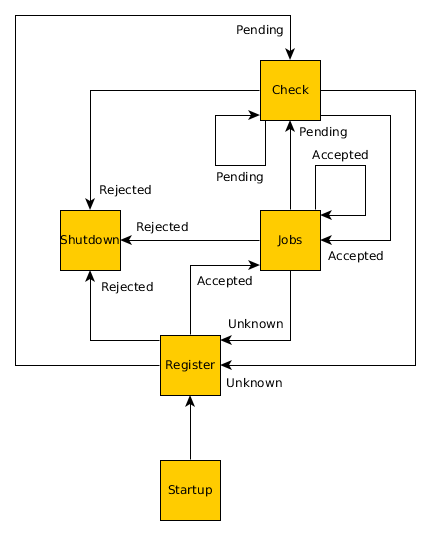
\includegraphics[width=\textwidth]{sa-states}
\centering
\caption{Οι πιθανές καταστάσεις του Software Agent και οι μεταβάσεις μεταξύ τους ανάλογα με τις απαντήσεις του Aggregator Manager.}
\end{figure}


\end{sloppypar}

\end{document}
